\documentclass{standalone}
\usepackage{tikz}
\usetikzlibrary{positioning, shapes.misc}

\begin{document}

\begin{tikzpicture}

% Placeholder image
\node[inner sep=0, outer sep=0] (image) at (0,0) {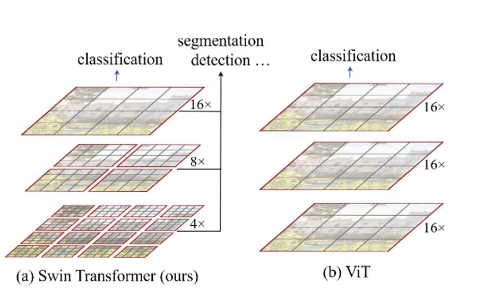
\includegraphics[width=15cm,height=8cm]{tikz/chapter8 - Swin Transformer.png}};
\node[fill=white, xshift=-4.6cm, yshift=-3.3cm, minimum width=8cm, minimum height=1cm] {};
\node[fill=white, xshift=-4.3cm, yshift=-3.2cm] {\Large Swin Transformer};
\node[fill=white, xshift=4.6cm, yshift=-3.3cm, minimum width=8cm, minimum height=1cm] {};
\node[fill=white, xshift=3.3cm, yshift=-3.2cm] {\Large ViT};

\node[fill=white, xshift=-3.8cm, yshift=2.8cm, minimum width=3cm, minimum height=1cm] {};
\node[fill=white, xshift=-3.8cm, yshift=2.5cm] {\large classification};
\node[fill=white, xshift=3.5cm, yshift=2.8cm, minimum width=3cm, minimum height=1cm] {};
\node[fill=white, xshift=3.5cm, yshift=2.5cm] {\large classification};

\node[fill=white, xshift=-0.5cm, yshift=2.62cm, minimum width=3cm, minimum height=1cm] {};
\node[fill=white, xshift=-0.5cm, yshift=2.4cm] {\large detection...};
\node[fill=white, xshift=-0.6cm, yshift=2.9cm] {\large segmentation};

\end{tikzpicture}

\end{document}